%!TEX root = ../dissertation.tex

\chapter{Introduction}
\label{chapter:introduction}
\section{Context and environment of the internship}

During my first semester of my international year, I have been doing a research internship in \gls{IST} in Lisbon, Portugal. This internship took place in \gls{ISR} which is part of \gls{IST}.

During this period I have been part of a robotic research team called SocRob that stands for Social Robotic (before it was for Soccer Robot). This team has a long history in robotic competitions, specially European Robotic League and RoboCup. I had the chance to participate to both of these competitions during my internship. SocRob was at the origin participating to these competitions with soccer robot: robots playing soccer against another robot team with the goal to score more points than the other team. After a few years, it was decided to participate in the same competitions but in an other league called: robot for home. Soccer robots were abandoned to a new robot called \gls{Mbot}.

\gls{Mbot}, is a robot designed at the origin to provide company and interaction to kids that have difficulties to have social interaction with humans (\ref{Mbot}). He was able to communicate through his screen and his face was showing emotions through the led systems on his "face" (eyes and mouth). He was able to play various game and activities with kids. The design was made by a company called IDMind. Six \glspl{Mbot} are still in activity in hospitals of the Lisbon area. The Monarch project reaching an end, Researchers working in \gls{ISR} decided to upgrade two \glspl{Mbot} to be able to participate to the home robotic league. \\[0.05cm]

\begin{figure} [!h]
    \centering
    \includegraphics[width=0.30\linewidth]{images/MBOT_01s.jpg}
    \caption{Mbot, as it was designed for Monarch Project}
    \label{Mbot}
\end{figure}
\newpage

Mbot was upgraded by the SocRob@Home team \ref{Mbot_upgraded} in \gls{ISR}. It was added a robotic arm (a Cython Gamma 1500) that has 7 \gls{DoF}. It was also upgraded in many others aspects, like adding an RGB-D camera on the head, having some speakers and a microphone to be able to speak and to understand people talking to him. Also, these hardware modifications have lead to software upgrade. Multiple research topics are experimented on Mbot in \gls{ISR}, for example : Natural Language Understanding, SLAM and navigation, people recognition and following. It's an awesome platform of field testing for researchers that is improving every year and that is being tested in robotic competitions. \\[0.05cm]

\begin{figure} [!h]
    \centering
    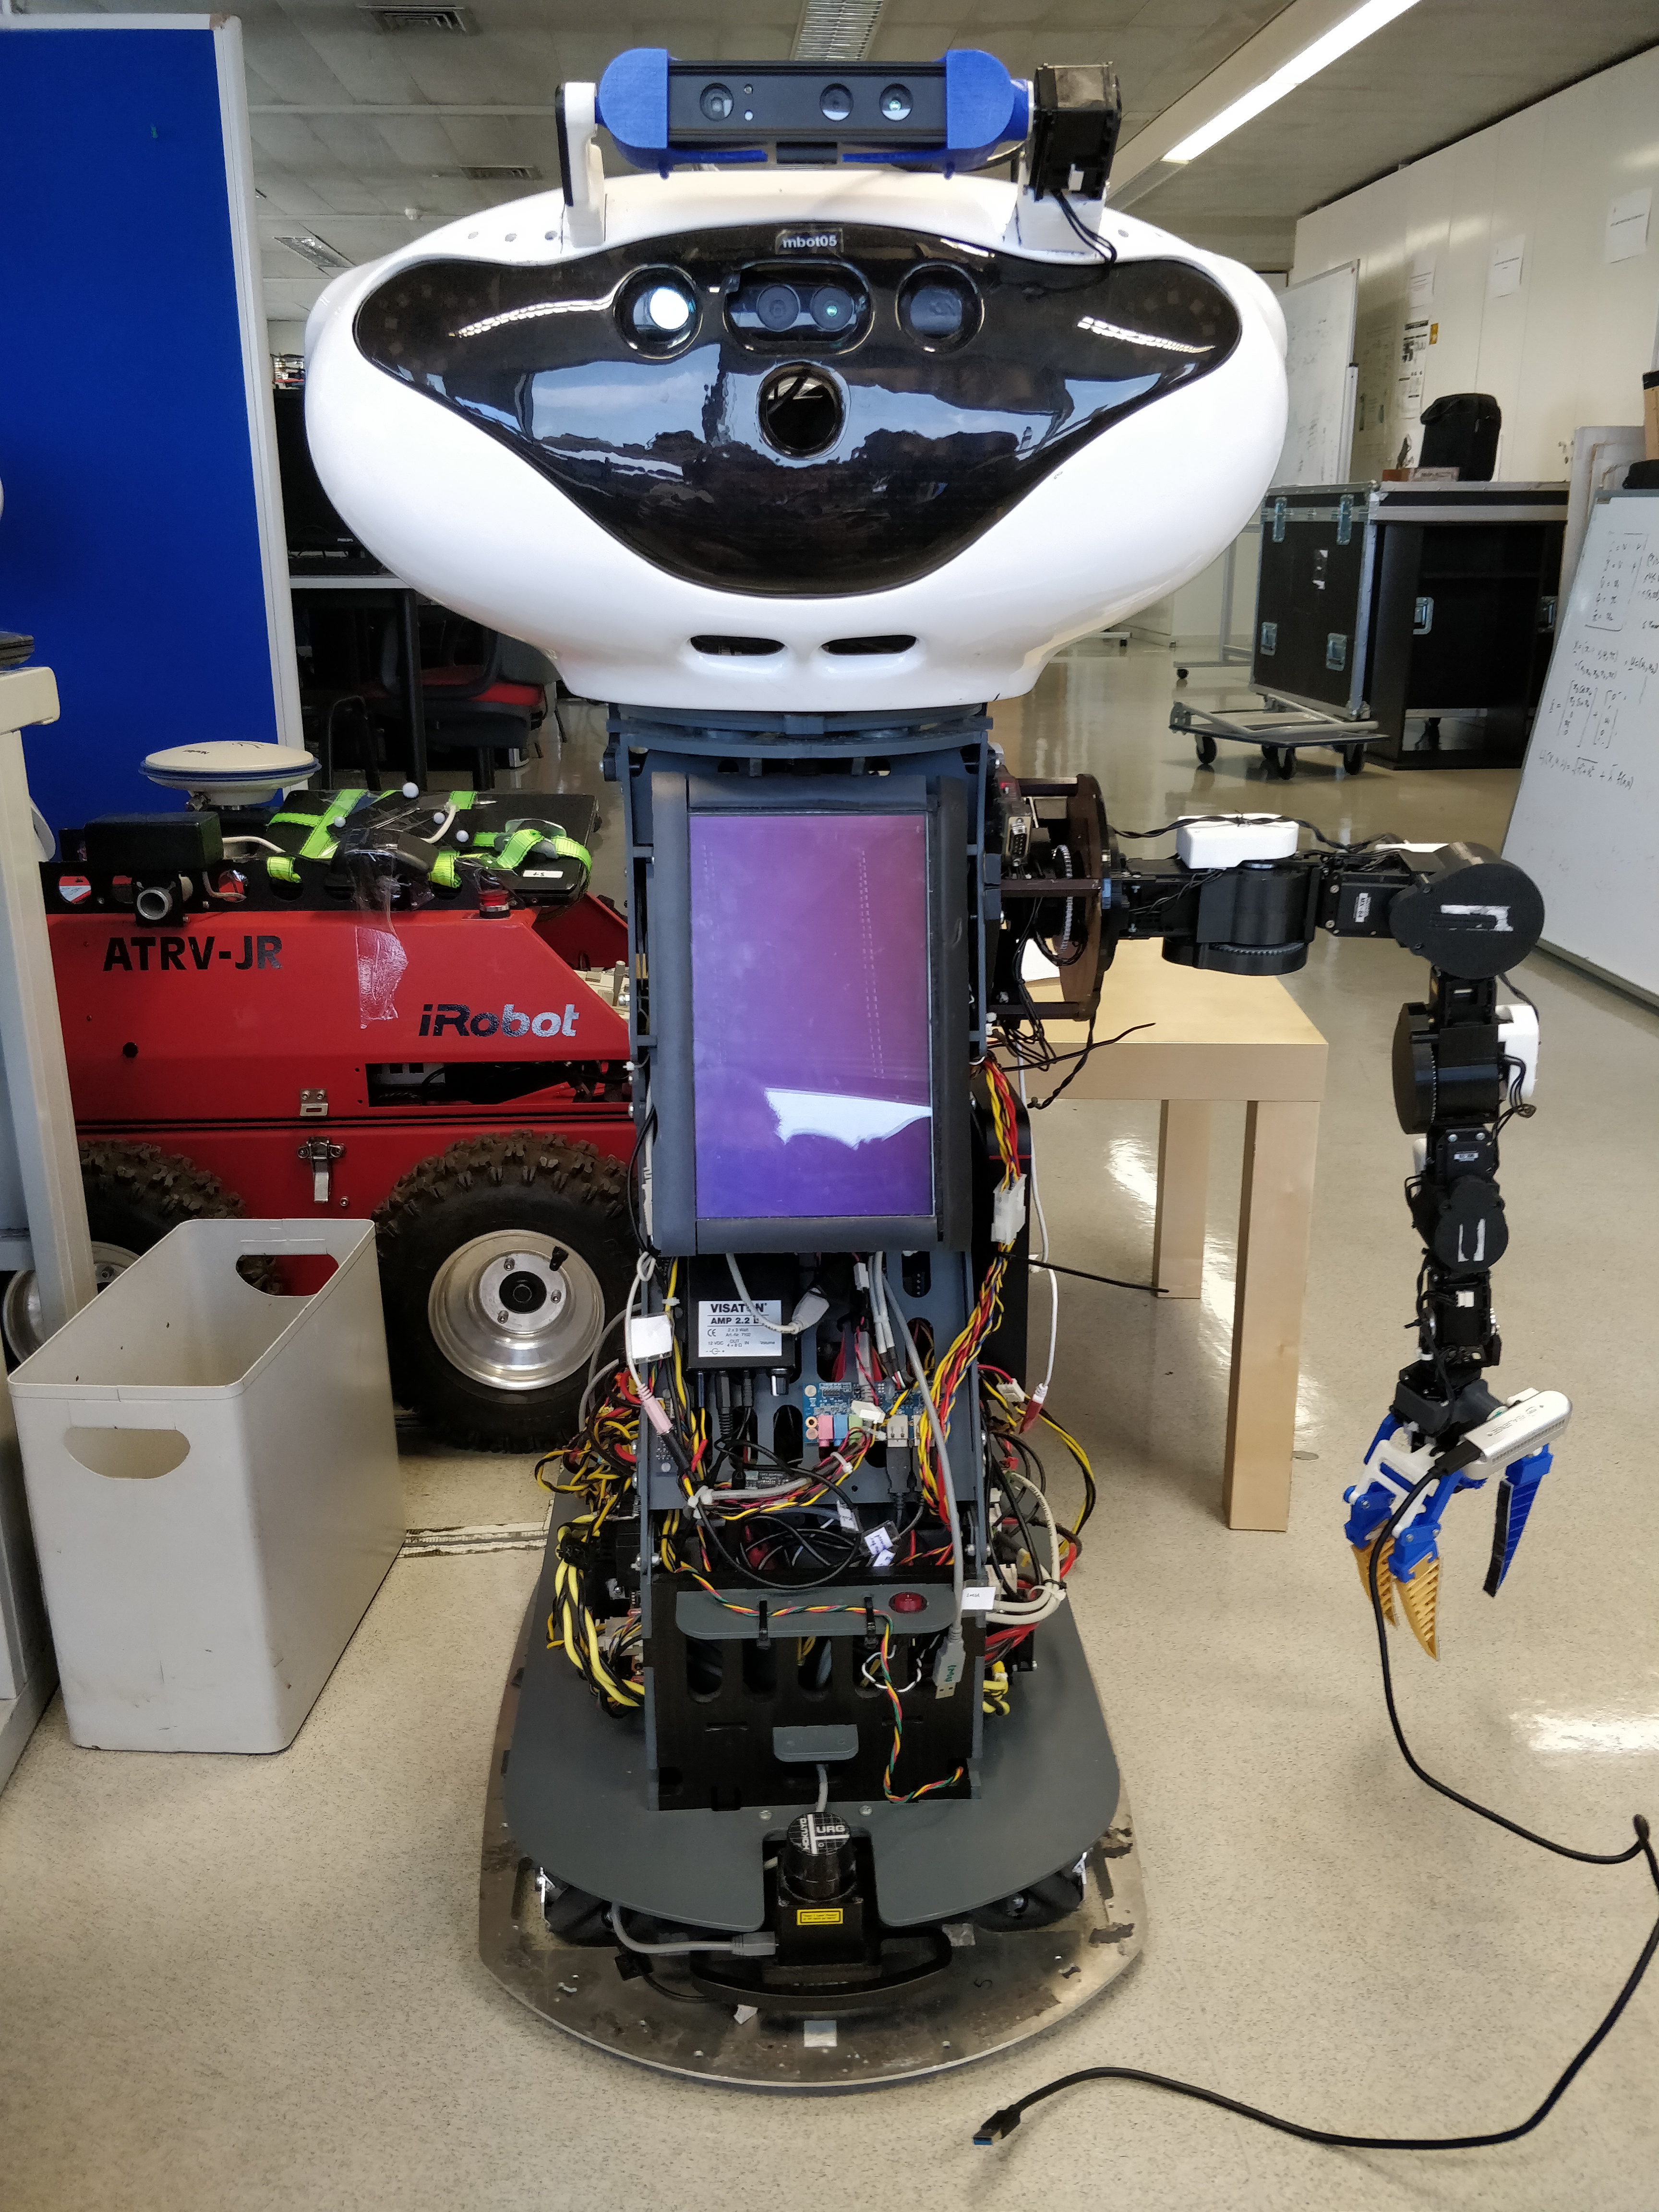
\includegraphics[width=0.35\linewidth]{images/IMG_20180908_165314.jpg}
    \caption{Mbot, upgraded by the SocRob@Home team}
    \label{Mbot_upgraded}
\end{figure}


My internship took place in this context of research and improvement on Mbot with the goal to test these improvements in robotic competitions. SocRob@Home team is composed by various type of researchers and students, there are some PhD students, some Master students and also some research engineers. During the time I was part of this team, the number of people varied from 5 to 15 peoples working on the robot. It is a relative big team for a university project and inside ISR, SocRob@Home was the biggest robotic team. Inside the SocRob@Home team, I was part of the manipulation team, that was composed by 3 or 4 people. This team is focused on interaction and manipulation of object with the arm of Mbot. I had the chance to participate with this team to RoboCup 2018 that took place in Montreal, Canada and a challenge of the European Robotic League, that took place in Madrid, Spain.\\[0.1cm]

The laboratory where my internship took place is at the 8th floor of the North tower in IST campus in Alameda \ref{IST}. It's the historical campus of IST. It's situated in the center of Lisbon. IST is one of the oldest university of Portugal and has also the status of engineering school that is unique in Portugal. It was founded in 1911 and it's the largest (6000 graduated students per year) and most prestigious engineering school of Portugal. \\[0.3cm]

\begin{figure} [!ht]
    \centering
    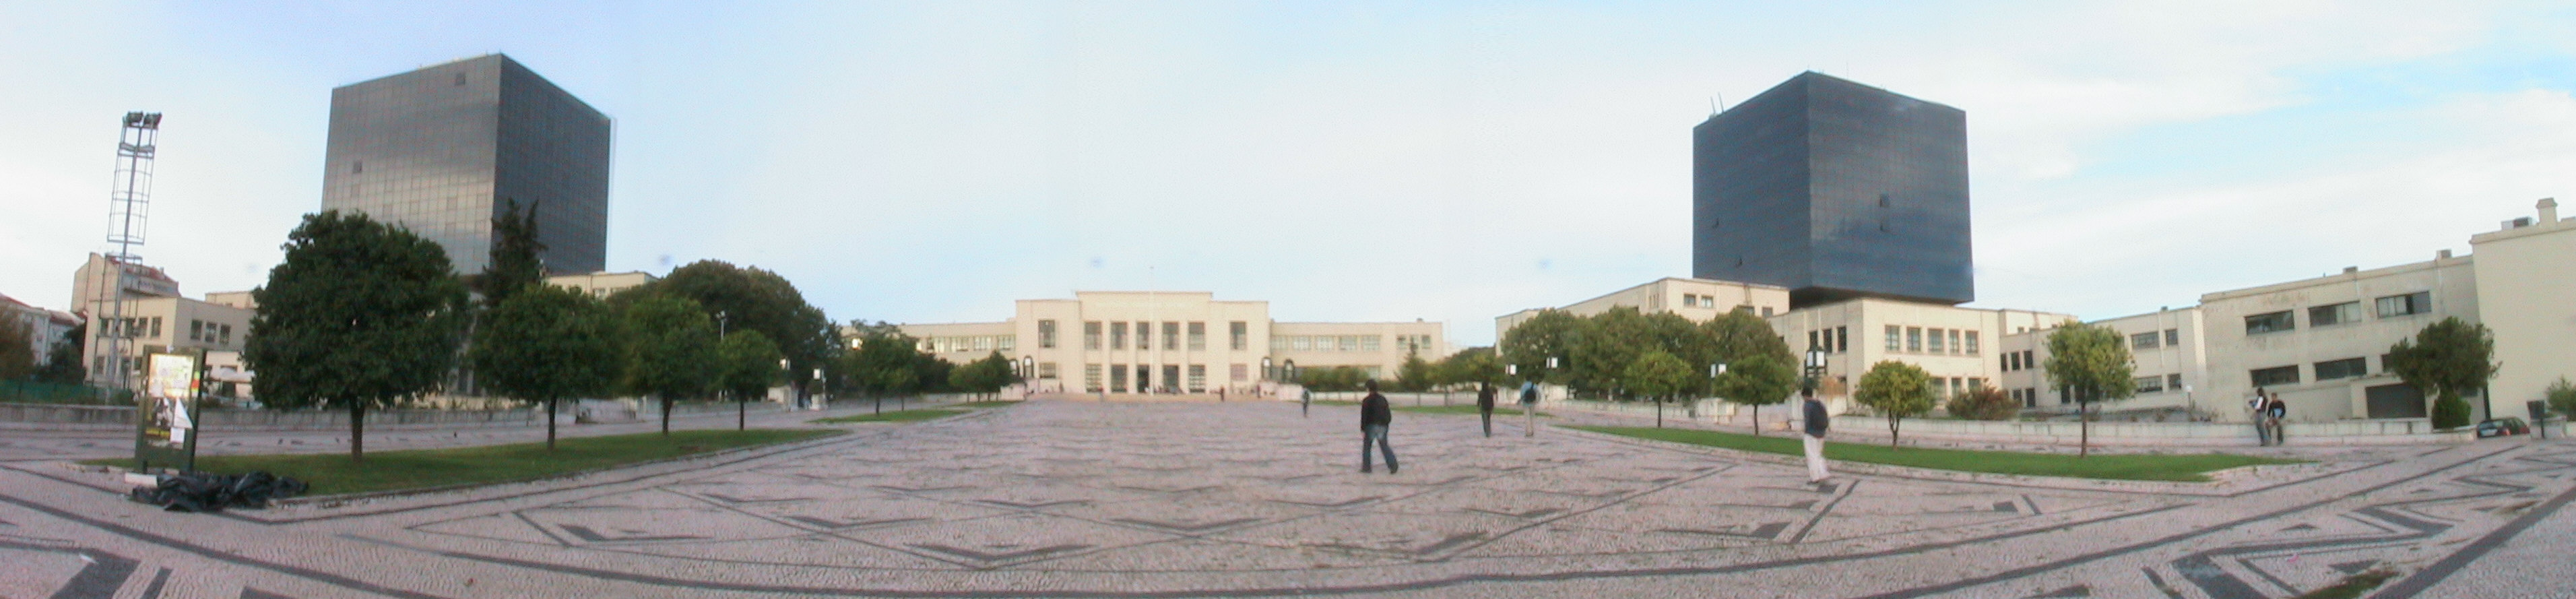
\includegraphics[width=1\linewidth]{images/panoramaIST.png}
    \caption{IST campus, on the right the North tower, Lisbon}
    \label{IST}
\end{figure}

The laboratory where I worked most of the time was very different from what I knew. It was a large area with multiple teams working at the time: one team working on a robot to assist fireman, on team on sub aquatic robotic and one team working on drones. For our team and to be able to work on a home environments, an entire flat was rebuild inside the laboratory with a kitchen, a bathroom, a room and a living room \ref{laboratory}. In this flat, robotic competitions are organized and It was a nice area to train the robot to work in a realistic home environment.\\[0.05cm]

\begin{figure} [!ht]
    \centering
    \includegraphics[width=0.8\linewidth]{images/41339074_481840472313432_6451621996257083392_n.jpg}
    \caption{SocRob@Home home laboratory}
    \label{laboratory}
\end{figure}


The subject of my internship was visual servoing on a 7\gls{DoF} arm. The goal is to control Mbot's arm with a  control law to make him able to grasp various types of object in various conditions.
In the next section, I am going to present my motivation and state the problem of my internship in this context and environment that we just presented.
\newpage


\section{Motivation}

Robust execution of complex manipulation tasks in dynamic environments is essential for service robots in domestic environments to assist their users in their daily tasks. By dynamic environment, I mean an environment that is changing, that could be known and unknown at the time (for the example the map of the apartment could be known but the position of the object to interact with could be unknown). Daily robotic tasks for a home robot on a manipulation side involve interaction with humans (shaking hands) and interaction with objects (taking an object from one position to a new one). Theses tasks involve the successful execution of multiple sub-tasks like object detection, grasping, carrying and placing objects.

Typically, object grasping problems are approached by using separate offline path planning and open loop execution methods, which expose some disadvantages. For instance, during trajectory execution, the robot is not sensitive to changes in the environment. If the target object pose is changed, the robot should ideally deal successfully with those situations and adjust accordingly. Having a control scheme that is closed loop will able the robot to adapt his movements to his dynamic environments.

A second problem when it comes to object grasping is related with robot base-camera-arm calibration. This work is motivated by the possibility of bypassing the calibration issues. Indeed, this work implied having a depth camera fixed on the end-effector and computing directly the visual control law in the image space, \gls{IBVS}.

A third problem is the variability of objects that the robot has to grasp. This work is motivated by the possibility to have a generic control law including a generic perception  for various types of objects and not restrained as a specific object.

\section{Problem Statement}

The problem is defined as the design and implementation of a generic real-time closed-loop image based visual servoing controller in a dynamic environment. This problem can be break down in three sub-sections: 

\begin{figure} [!h]
    \begin{minipage}[b]{0.5\linewidth}
        \begin{enumerate}
            \item Perception
            \begin{enumerate}
                \item Detection
                \item Features Extraction
                \item Tracking 
            \end{enumerate}
                \item Control Law
            \begin{enumerate}
                \item \gls{IBVS}
            \end{enumerate}
            \item Execution
            \begin{enumerate}
                \item Arm controller
            \end{enumerate}
        \end{enumerate}
    \end{minipage}
    \begin{minipage}[b]{0.5\linewidth}
      \begin{center}
        \includegraphics[width=0.8\textwidth]{images/mbot_grasping.png}
      \end{center}
      \caption{Mbot, in a grasping approach}
    \end{minipage}
\end{figure}

\newpage


This method has been applied for a domestic robots in a domestic environment. It has been both implemented in simulation and inside the real robot.

The closed loop controller take as input image, where characteristic features of the desired grasping object are extracted, with a perception part that has been developed from state of the art solutions. The camera velocities are computed as output since the camera is directly fixed on the end-effector we can assume that the end effector velocities are computed. 


\section{Report Outline}

This work has the following structures: Chapter \ref{chapter:Background} provides a state of the art review combined with background information required to understand the proposed solution. Chapter \ref{chapter:Implementation} presents the new approach, the implementation in simulation and inside the robot. Chapter \ref{chapter:conclusion} summarizes the achievements and discuss about future works. This chapter will also include a quick overview of the Portuguese life as requested. 
